% ============================================================================
% Pedagogical solutions - Practice 6 (Combinations & multinomials).
% English, pdflatex. ASCII-clean source (no em-dash, no " -- ", no straight ").
% Compile: pdflatex twice, then view the PDF.
% ============================================================================
\documentclass[11pt,a4paper]{article}

% ---- Encoding & fonts ----
\usepackage[utf8]{inputenc}
\usepackage[T1]{fontenc}
\usepackage{lmodern}

% ---- Math ----
\usepackage{amsmath,amssymb,amsthm}
\usepackage{mathtools}

% ---- Layout ----
\usepackage[margin=2.3cm]{geometry}
\usepackage{enumitem}
\usepackage{booktabs}
\usepackage{array}

% ---- Visuals ----
\usepackage{xcolor}
\usepackage[most]{tcolorbox}
\usepackage{tikz}
\usetikzlibrary{arrows.meta,positioning,calc,fit,backgrounds,shapes.misc}
\usepackage{pgfplots}
\pgfplotsset{compat=1.18}
\usepackage{hyperref}
\hypersetup{colorlinks=true,linkcolor=blue!55!black,urlcolor=blue!55!black}

% ---- Palette (Armenian flag colours; use for 3+ series plots) ----
\definecolor{armRed}{HTML}{D90012}
\definecolor{armBlue}{HTML}{0033A0}
\definecolor{armOrange}{HTML}{F2A800}
\definecolor{ink}{HTML}{22303C}

\setlength{\parindent}{0pt}
\setlength{\parskip}{5pt}

% ---- Boxes ----
\newtcolorbox{problembox}[1][]{enhanced, breakable, sharp corners=south,
  colback=armOrange!10, colframe=armOrange!75!black, boxrule=0.8pt, arc=2mm,
  fonttitle=\bfseries\color{white}, coltitle=white,
  attach boxed title to top left={xshift=4mm,yshift=-2.4mm},
  boxed title style={colback=armOrange!85!black, arc=1mm},
  title={Problem #1}}

\newtcolorbox{ideabox}{enhanced, breakable,
  colback=armBlue!6, colframe=armBlue!70!black, boxrule=0.8pt, arc=2mm,
  fonttitle=\bfseries\color{white}, coltitle=white,
  attach boxed title to top left={xshift=4mm,yshift=-2.4mm},
  boxed title style={colback=armBlue!75!black, arc=1mm},
  title={The idea}}

\newtcolorbox{methodbox}{enhanced, breakable,
  colback=gray!8, colframe=gray!55!black, boxrule=0.7pt, arc=2mm,
  fonttitle=\bfseries, title={$\bigstar$\ Method to remember}}

\newtcolorbox{answerbox}{enhanced, sharp corners=south,
  colback=green!8, colframe=green!50!black, boxrule=1pt, arc=2mm, left=4mm,right=4mm}
\newcommand{\answer}[1]{\begin{answerbox}\centering\textbf{Answer:}\quad #1\end{answerbox}}

% ---- Title ----
\title{\vspace{-1.2cm}\textbf{Discrete Mathematics - Practical 6}\\[2pt]
\large Combinations, binomial and multinomial coefficients: worked solutions\\[2pt]
\normalsize\itshape with the reasoning spelled out, step by step}
\author{}
\date{}

\begin{document}
\maketitle
\vspace{-1.0cm}

\section*{Warm-up}
This sheet is about \emph{counting selections and arrangements}. The whole chapter rests on
four reusable ideas: the \textbf{product rule} (independent choices multiply), \textbf{combinations}
$\binom{n}{r}$ (choose an unordered $r$-subset of $n$ items), \textbf{combinations with repetition}
(distribute identical items into labelled boxes, a.k.a. stars and bars), and the
\textbf{multinomial coefficient} $\frac{n!}{n_1!\,n_2!\cdots}$ (arrange a multiset where some items
repeat). The art is recognising which model a word problem secretly is. Below we solve problems 8,
9 and 11, and for each we first explain \emph{why} the chosen model fits before turning the crank.

% ============================================================================
\section*{Problem 8 - Lattice paths through a checkpoint}

\begin{problembox}[8]
In the integer grid, count the monotone paths from $O(0,0)$ to $A(7,8)$ that pass through the
point $(3,4)$. Each step goes one unit \textbf{right} or one unit \textbf{up}.
\end{problembox}

\begin{ideabox}
First, why are monotone paths counted by a binomial coefficient at all? To get from $O(0,0)$ to
$A(7,8)$ using only right ($R$) and up ($U$) steps, you must take exactly $7$ rights and $8$ ups,
in \emph{some order}. So a path \textbf{is} a word of $7$ $R$'s and $8$ $U$'s, a sequence of
$7+8=15$ steps. To build one you only have to decide which $7$ of the $15$ slots hold the $R$'s (the
remaining slots are forced to be $U$'s) - that is $\binom{15}{7}$ choices. Counting paths becomes
counting where the rights go.

Now the checkpoint. Any path through $(3,4)$ splits cleanly into two halves: the journey
$O\to(3,4)$, then the journey $(3,4)\to A$. These two halves are \textbf{independent} (whatever you
do before $(3,4)$ does not restrict what you do after), so by the product rule we multiply the count
of first halves by the count of second halves. The checkpoint turns one hard count into two easy
ones.
\end{ideabox}

\textbf{Step 1 - First leg $O(0,0)\to(3,4)$.}
This leg needs $3$ rights and $4$ ups, so $3+4=7$ steps. A path is a choice of which $3$ of those
$7$ steps are the rights:
$$\binom{7}{3}=\frac{7!}{3!\,4!}=35.$$

\textbf{Step 2 - Second leg $(3,4)\to A(7,8)$.}
This leg needs $7-3=4$ rights and $8-4=4$ ups, so $8$ steps. Choose which $4$ are rights:
$$\binom{8}{4}=\frac{8!}{4!\,4!}=70.$$

\textbf{Step 3 - Multiply (product rule).}
$$\binom{7}{3}\binom{8}{4}=35\cdot 70=2450.$$

\textbf{Always check.} A sanity bound: the \emph{total} number of $O\to A$ paths (ignoring the
checkpoint) is $\binom{15}{7}=6435$, and our answer $2450$ is comfortably less, as it must be since
not every path visits $(3,4)$. Also the split is consistent: $35\cdot 70 = 2450$, and a direct
computer enumeration of all $6435$ paths finds exactly $2450$ passing through $(3,4)$.

\answer{$\displaystyle \binom{7}{3}\binom{8}{4}=35\cdot 70=2450$}

\begin{methodbox}
\textbf{Transferable technique - paths and the checkpoint split.} A monotone grid path from
$(0,0)$ to $(a,b)$ corresponds to a word of $a$ rights and $b$ ups, so there are $\binom{a+b}{a}$ of
them. To force a path through a fixed point $P$, cut it at $P$ and \textbf{multiply} the count of
the two independent legs. \textbf{To forbid} a point, subtract: (paths through $P$) from the total.
\end{methodbox}

\medskip
\textbf{Seeing the split.} The grid below shows the two legs. Each leg is its own little
path-counting problem; the checkpoint $(3,4)$ welds them together.

\begin{center}
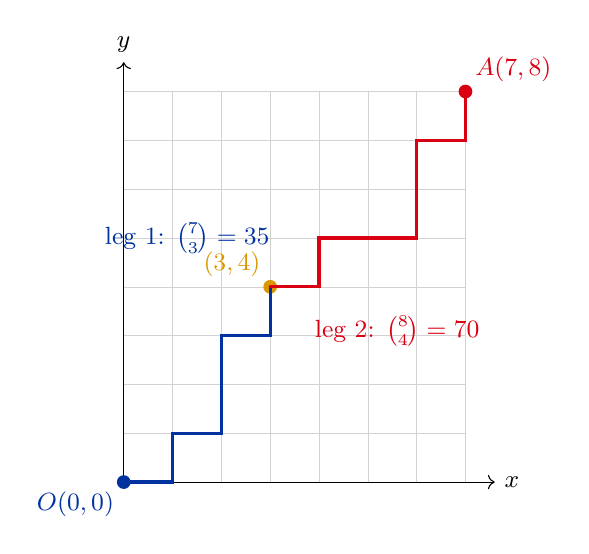
\begin{tikzpicture}[scale=0.62, font=\small]
  % grid
  \draw[step=1, gray!35, very thin] (0,0) grid (7,8);
  \draw[->] (0,0) -- (7.6,0) node[right]{$x$};
  \draw[->] (0,0) -- (0,8.6) node[above]{$y$};
  % key points
  \fill[armBlue] (0,0) circle (4pt) node[below left]{$O(0,0)$};
  \fill[armOrange!90!black] (3,4) circle (4pt) node[above left]{$(3,4)$};
  \fill[armRed] (7,8) circle (4pt) node[above right]{$A(7,8)$};
  % a sample first leg O->(3,4)
  \draw[armBlue, very thick, line cap=round]
     (0,0) -- (1,0) -- (1,1) -- (2,1) -- (2,2) -- (2,3) -- (3,3) -- (3,4);
  % a sample second leg (3,4)->A
  \draw[armRed, very thick, line cap=round]
     (3,4) -- (4,4) -- (4,5) -- (5,5) -- (6,5) -- (6,6) -- (6,7) -- (7,7) -- (7,8);
  \node[armBlue]  at (1.3,5.0) {leg 1: $\binom{7}{3}=35$};
  \node[armRed]   at (5.6,3.1) {leg 2: $\binom{8}{4}=70$};
\end{tikzpicture}
\end{center}

% ============================================================================
\section*{Problem 9 - Decompositions of 6 into three summands}

\begin{problembox}[9]
Count the number of ways to write $6$ as a sum of three summands.
\end{problembox}

\begin{ideabox}
The word \emph{decomposition} (\emph{trohum}) on its own can mean an \emph{unordered} partition,
so the count genuinely depends on the convention. This exercise sits in the \textbf{combinations
with repetition} section, which fixes the reading: the three summands are \textbf{ordered} (first,
second and third place are distinct) and \textbf{zero is allowed}, exactly as in the lecture example where
$4=x_1+x_2$ was counted as $5$ ways: $4{+}0,\,3{+}1,\,2{+}2,\,1{+}3,\,0{+}4$. So we are counting the
integer solutions of
$$x_1+x_2+x_3=6,\qquad x_i\ge 0.$$
Why is this a \textbf{stars and bars} problem? Picture the $6$ as six identical stars in a row.
Choosing the three summands is the same as dropping \textbf{two bars} among the stars to cut the row
into three groups: the stars before the first bar are $x_1$, between the bars $x_2$, after the second
bar $x_3$. Empty groups are allowed (two bars can be adjacent, giving a zero summand). Every
placement of the two bars gives exactly one solution, and vice versa, so we just count bar
placements.
\end{ideabox}

\textbf{Step 1 - Encode as a row of symbols.}
Lay out $6$ stars and $2$ bars in a line, e.g. $\star\star\,|\,\star\,|\,\star\star\star$, which reads
$x_1=2,\ x_2=1,\ x_3=3$. The whole row has $6+2=8$ symbol positions.

\textbf{Step 2 - Count the arrangements.}
A solution is fixed once we decide which $2$ of the $8$ positions are the bars (the rest are stars):
$$\binom{6+3-1}{3-1}=\binom{8}{2}=\frac{8\cdot 7}{2}=28.$$

\textbf{Always check.} Direct count of solutions of $x_1+x_2+x_3=6$ with $x_i\ge0$: as $x_1$ runs
from $0$ to $6$, the remaining $x_2+x_3=6-x_1$ has $(6-x_1)+1$ solutions, giving
$7+6+5+4+3+2+1=28$. A brute-force triple loop also returns $28$. \checkmark

\answer{$\displaystyle \binom{8}{2}=28$}

\begin{methodbox}
\textbf{Transferable technique - stars and bars.} The number of ordered nonnegative integer
solutions of $x_1+\dots+x_k=n$ is $\binom{n+k-1}{k-1}$ (place $k-1$ bars among $n$ stars). This is
\emph{combinations with repetition}: it equals the number of ways to choose a multiset of size $n$
from $k$ types. If instead each $x_i\ge 1$, first hand one unit to each variable, then solve
$x_1'+\dots+x_k'=n-k$, giving $\binom{n-1}{k-1}$.
\end{methodbox}

\medskip
\textbf{The bars picture.} Three sample placements of the two bars among six stars:

\begin{center}
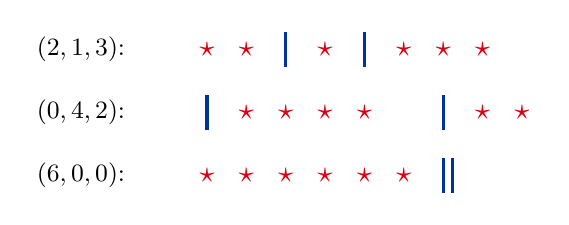
\begin{tikzpicture}[font=\small, star/.style={armRed, scale=1.2}, bar/.style={armBlue, very thick}]
  % row 1: 2|1|3
  \node at (-1.6,0) {$(2,1,3)$:};
  \foreach \x in {0,1} {\node[star] at (\x*0.5,0) {$\star$};}
  \draw[bar] (1.0,-0.22) -- (1.0,0.22);
  \node[star] at (1.5,0) {$\star$};
  \draw[bar] (2.0,-0.22) -- (2.0,0.22);
  \foreach \x in {0,1,2} {\node[star] at (2.5+\x*0.5,0) {$\star$};}
  % row 2: 0|4|2
  \node at (-1.6,-0.8) {$(0,4,2)$:};
  \draw[bar] (0.0,-0.8-0.22) -- (0.0,-0.8+0.22);
  \foreach \x in {0,1,2,3} {\node[star] at (0.5+\x*0.5,-0.8) {$\star$};}
  \draw[bar] (3.0,-0.8-0.22) -- (3.0,-0.8+0.22);
  \foreach \x in {0,1} {\node[star] at (3.5+\x*0.5,-0.8) {$\star$};}
  % row 3: 6|0|0
  \node at (-1.6,-1.6) {$(6,0,0)$:};
  \foreach \x in {0,1,2,3,4,5} {\node[star] at (\x*0.5,-1.6) {$\star$};}
  \draw[bar] (3.0,-1.6-0.22) -- (3.0,-1.6+0.22);
  \draw[bar] (3.12,-1.6-0.22) -- (3.12,-1.6+0.22);
\end{tikzpicture}
\end{center}
Adjacent bars (last row) produce zero summands, which is why $\binom{8}{2}=28$ and not the smaller
$\binom{5}{2}=10$ that the all-positive convention would give.

% ============================================================================
\section*{Problem 11 - Arrangements of the letters of a word}

\begin{problembox}[11]
How many distinct \textquotedbl{}words\textquotedbl{} (orderings of all the letters) can be formed
from the letters of the Armenian word \textbf{matematika} (the original is in Armenian script; by
sound its ten letters are m-a-t-e-m-a-t-i-k-a)?
\end{problembox}

\begin{ideabox}
If all $10$ letters were \emph{different}, the answer would simply be $10!$ orderings. The twist is
that some letters \textbf{repeat}, and swapping two copies of the same letter does not produce a new
visible word. So $10!$ over-counts: it treats the repeated copies as if they were distinguishable.

The fix is to \textbf{divide out} the over-counting. If a letter appears $m$ times, then for every
genuinely distinct word the $10!$ count secretly lists it $m!$ times (one for each way of permuting
those identical copies among their slots). Dividing by $m!$ for each repeated letter removes exactly
that redundancy. This ratio is the \textbf{multinomial coefficient}.

\textbf{The crucial counting step is getting the multiset right - and here we must count Armenian
letters, not the Latin transliteration.} The word has two different \textquotedbl{}t\textquotedbl{}
sounds that are \emph{distinct Armenian letters}: the aspirated one (Armenian
\textquotedbl{}t'\textquotedbl{}, in \textbf{matematika} the third letter) and the plain one
(Armenian \textquotedbl{}t\textquotedbl{}, the seventh letter). Each appears only \emph{once}, so
they are \textbf{not} a repeated letter. Confusing them (as the Latin spelling \texttt{matematika}
would, with its two identical \texttt{t}'s) gives the wrong answer.
\end{ideabox}

\textbf{Step 1 - List the multiset of letters.}
Writing the ten Armenian letters in order and grouping equal ones:
\begin{center}
\small
\begin{tabular}{@{}lcl@{}}
\toprule
letter (Armenian, by sound) & count & note\\
\midrule
m  & $2$ & repeated\\
a  & $3$ & repeated\\
t' (aspirated t) & $1$ & a distinct letter\\
e  & $1$ &\\
t  (plain t) & $1$ & a \emph{different} distinct letter\\
i  & $1$ &\\
k  & $1$ &\\
\bottomrule
\end{tabular}
\end{center}
Total $2+3+1+1+1+1+1=10$ letters. Only \textbf{m} (twice) and \textbf{a} (three times) repeat.

\textbf{Step 2 - Apply the multinomial coefficient.}
$$\frac{10!}{2!\,3!\,1!\,1!\,1!\,1!\,1!}=\frac{10!}{2!\,3!}
   =\frac{3\,628\,800}{2\cdot 6}=\frac{3\,628\,800}{12}=302\,400.$$

\textbf{Always check.} Two independent checks.
\emph{(i) Build the word by placing letters into the $10$ slots.} Choose the $2$ slots for the
\textbf{m}'s: $\binom{10}{2}=45$. From the remaining $8$ slots choose the $3$ for the \textbf{a}'s:
$\binom{8}{3}=56$. The last $5$ distinct letters fill the remaining $5$ slots in $5!=120$ ways. Then
$45\cdot 56\cdot 120 = 302\,400$, matching. \emph{(ii)} A computer enumeration of the distinct
permutations of the multiset returns exactly $302\,400$.

\answer{$\displaystyle \frac{10!}{2!\,3!}=302\,400$}

\medskip
\textbf{Why the letter count matters.} If one wrongly used the Latin spelling \texttt{matematika},
the two \texttt{t}'s would merge into one repeated letter and the count would drop to
$$\frac{10!}{2!\,2!\,3!}=151\,200,$$
which is exactly half. The factor of $2$ is the $2!$ for the (false) pair of identical t's. The
problem is about the Armenian spelling, where the two t-letters are distinct, so the answer is
$302\,400$.

\begin{methodbox}
\textbf{Transferable technique - permutations of a multiset.} To arrange $n$ items where the
distinct types occur with multiplicities $n_1,n_2,\dots,n_r$ (so $\sum n_i=n$), the number of
distinct orderings is the multinomial coefficient
$$\binom{n}{n_1,n_2,\dots,n_r}=\frac{n!}{n_1!\,n_2!\cdots n_r!}.$$
Start from $n!$ (all items distinct), then divide by $n_i!$ for each type to cancel the
indistinguishable permutations of its copies. The single most error-prone step is reading the
multiset correctly: count what is \emph{actually} the same symbol, not what looks similar in a
transliteration.
\end{methodbox}

\medskip
\textbf{Counting the same word with three methods (all agree).}

\begin{center}
\small
\begin{tabular}{@{}lll@{}}
\toprule
method & computation & value\\
\midrule
multinomial          & $10!/(2!\,3!)$                        & $302\,400$\\
slot-filling         & $\binom{10}{2}\binom{8}{3}\,5!=45\cdot56\cdot120$ & $302\,400$\\
direct enumeration   & count distinct multiset permutations  & $302\,400$\\
\bottomrule
\end{tabular}
\end{center}

\end{document}
